\subsection{Niveau 3 - Timer}

\begin{center}
\begin{figure}[!h]
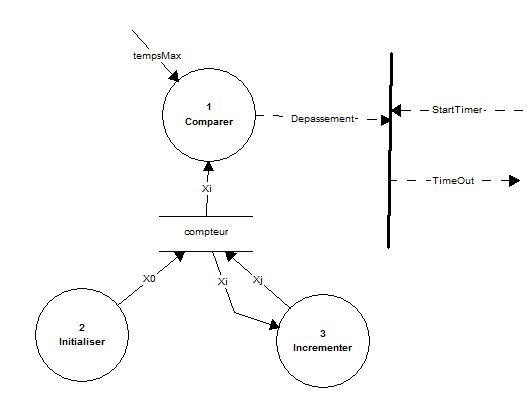
\includegraphics[height=11cm]{\PIXPATH/timer}
\caption{Niveau 3 - Timer}
\end{figure}
\end{center}


\subsubsection{Diagramme états-transitions}

\begin{center}
\begin{figure}[!h]
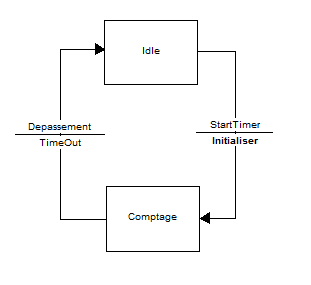
\includegraphics[height=7cm]{\PIXPATH/timer_etat}
\caption{Diagramme états-transitions}
\end{figure}
\end{center}

\subsubsection{Processus primitifs - C-Spec}

\begin{description}
	
	\item \textbf{Comparer}
		\begin{tabbing} 
		\textbf{IN} : tempsMax, Xi \\
		\textbf{OUT} : Depassement\\
		si \=($tempsMax \leq Xi$) \\
			\>Depassement emis \\
		fin si 
		\end{tabbing}

	\item \textbf{Initialiser}
		\begin{tabbing} 
		\textbf{IN} : X0 \\
		X0 : 0
		\end{tabbing}

	\item \textbf{Incrementer}
		\begin{tabbing} 
		\textbf{IN} : Xi \\
		\textbf{OUT} : Xj \\
		$Xj : Xi + 1$
		\end{tabbing}


\end{description}

\vfill
\pagebreak

